% Artigo — Template SBC (Sociedade Brasileira de Computação)
\documentclass[12pt]{article}
\usepackage[utf8]{inputenc}
\usepackage[T1]{fontenc}
\usepackage[brazil]{babel}
\usepackage{sbc-template}
\usepackage{graphicx}
\usepackage{url}
\usepackage{booktabs}
\usepackage{siunitx}
\sisetup{group-separator={.}, group-minimum-digits=4, output-decimal-marker={,}}

\sloppy

\title{Contratações de Nuvem nas Autarquias do MEC:\\Diagnóstico Empírico com Dados do PNCP}

\author{Luiz F. P. Quirino\inst{1}}

\address{Coordenadoria de Contratações Estratégicas de TI (CCETI-DTI)\\
  Instituto Federal de Educação, Ciência e Tecnologia de São Paulo (IFSP)\\
  São Paulo -- SP -- Brasil
  \email{luiz.quirino@ifsp.edu.br}
}

\begin{document}

\maketitle

\begin{abstract}
This paper presents an exploratory analysis of cloud computing service procurement practices across 196 federal agencies linked to Brazil's Ministry of Education (MEC). Using public data from the National Public Procurement Portal (PNCP) API, we analyzed 64,295 procurement processes (2022--2026), identifying 314 cloud-related processes from 88 institutions. Results reveal a predominance of direct contracting (61.5\%), with competitive bidding yielding 3.5$\times$ greater cost savings (18.3\% vs. 5.3\%). We identify 14 institutions with recurring direct-contracting patterns for cloud services (R\$ 11.5M across multiple waivers per fiscal year) and significant data quality issues in the PNCP (12.1\% missing homologation values). The analysis provides empirical evidence for preliminary technical studies and contributes to digital governance literature.
\end{abstract}

\begin{resumo}
Este artigo apresenta uma análise exploratória das práticas de contratação de serviços de computação em nuvem pelas 196 autarquias federais vinculadas ao Ministério da Educação (MEC). Utilizando dados da API do Portal Nacional de Contratações Públicas (PNCP), analisamos 64.295 processos (2022--2026), identificando 314 relacionados a nuvem em 88 instituições. Os resultados revelam predominância de contratação direta (61,5\%), com licitações competitivas gerando economia 3,5$\times$ superior (18,3\% vs. 5,3\%). Identificamos 14 instituições com padrões recorrentes de contratação direta para nuvem no mesmo exercício fiscal (R\$ 11,5 milhões em dispensas acumuladas) e problemas significativos de qualidade dos dados no PNCP (12,1\% sem valor de homologação). A análise fornece evidências empíricas para estudos técnicos preliminares e contribui para a literatura sobre governança digital.
\end{resumo}

\section{Introdução}
\label{sec:intro}

A computação em nuvem consolidou-se como plataforma central de suporte à transformação digital no setor público, permitindo ampliar capacidade de processamento, reduzir custos de infraestrutura e aprimorar escalabilidade \cite{mell2011nist}. No contexto governamental brasileiro, a Lei nº 14.133/2021 introduziu instrumentos de planejamento adequados a tecnologias emergentes, integrando gestão por resultados e análise de riscos \cite{brasil2021lei14133}. O Decreto nº 10.947/2022 e as Instruções Normativas da SGD detalham critérios para contratações de TIC, incluindo nuvem como modalidade preferencial.

Apesar da evolução normativa, não existe um panorama empírico consolidado sobre como as autarquias do MEC contratam nuvem. Iniciativas de consolidação já existem em múltiplas escalas: o ``Nuvem 3.0'' da SGD/MGI (contratação centralizada multicloud para o SISP), a Nuvem de Governo do Serpro (infraestrutura soberana) e credenciamentos conduzidos por autarquias individuais. Todas, porém, carecem de um diagnóstico empírico do cenário que pretendem transformar. Este estudo busca preencher essa lacuna, respondendo às seguintes questões de pesquisa:

\begin{itemize}
\item \textbf{QP1:} Qual o custo de oportunidade da contratação direta em comparação com certames competitivos?
\item \textbf{QP2:} Há padrões de recorrência de dispensas que indiquem oportunidades de consolidação via modalidades competitivas?
\item \textbf{QP3:} Qual a qualidade dos dados registrados no PNCP para fins de auditoria e transparência?
\item \textbf{QP4:} A especificidade técnica dos Termos de Referência influencia a economicidade obtida?
\end{itemize}

Para tanto, utilizamos dados extraídos da API pública do PNCP (art. 174, Lei 14.133/2021), analisando 64.295 processos de 196 autarquias entre 2022 e 2026. As contribuições são: (i) primeiro diagnóstico empírico das contratações de nuvem no MEC; (ii) quantificação do diferencial de economicidade entre modalidades; (iii) mapeamento de padrões de recorrência em contratações diretas; e (iv) avaliação da qualidade dos dados do PNCP como instrumento de transparência.

\section{Trabalhos Relacionados}
\label{sec:relacionados}

\subsection{Computação em nuvem e contratações no setor público}

A computação em nuvem transformou a gestão de infraestrutura digital no setor público \cite{mell2011nist}. Armbrust et al. \cite{armbrust2010above} identificaram que a elasticidade e o modelo \textit{pay-per-use} ofereciam vantagens para organizações com demanda variável. Revisões recentes confirmam a expansão da adoção governamental: Hashemi e Zarei \cite{hashemi2024cloud_security} identificaram segurança e privacidade como 70\% das barreiras, enquanto Pinheiro \cite{pinheiro2020cloudgov} evidenciou escassa atenção à dimensão contratual e econômica na literatura.

No contexto europeu, Cheng et al. \cite{cheng2017uk_cloud} identificaram riscos de \textit{vendor lock-in} em migrações governamentais. Lund et al. \cite{sweden_cloud2022} encontraram desafios semelhantes na Suécia. Nos EUA, o programa FedRAMP \cite{itif2020fedramp} padroniza certificação de provedores, e o GAO \cite{gao2024cloud} reportou lacunas na implementação de \textit{procurement} de nuvem mesmo com diretrizes estabelecidas.

No Brasil, a Lei nº 14.133/2021 \cite{brasil2021lei14133} modernizou o regime de licitações, e a Portaria SGD/MGI nº 5.950/2023 \cite{brasil2023portaria5950} estabelece o modelo específico para nuvem. Nogueira \cite{nogueira2021contratacoes} evidenciou carência de metodologias padronizadas de ETP. Barros \cite{barros2019governanca} concluiu que a desintegração entre planejamento estratégico e contratações é obstáculo central em universidades federais. O TCU, via Acórdão 1.503/2020 \cite{tcu2020acordao1503}, recomenda SRP e contratações conjuntas para nuvem.

\subsection{Auditoria, dados abertos e economicidade}

Baldi e Vannoni \cite{baldi2018econometric} forneceram evidência econométrica sobre economia em contratos competitivos nas Forças Armadas espanholas. Decarolis et al. \cite{decarolis2023bureaucratic} demonstraram que competência burocrática reduz atrasos e estouros de custos. No Brasil, Gonçalves, Santos e Quirino \cite{goncalves2026deteccao} aplicaram \textit{machine learning} para detecção de anomalias em contratações com dados abertos.

\subsection{Posicionamento}

A Tabela~\ref{tab:comparativo} sintetiza o posicionamento deste estudo.

\begin{table}[ht]
\centering
\caption{Quadro comparativo de trabalhos relacionados}
\label{tab:comparativo}
\footnotesize
\begin{tabular}{p{2cm}p{1.7cm}p{1.4cm}p{2.8cm}p{2.8cm}}
\toprule
\textbf{Estudo} & \textbf{Método} & \textbf{Recorte} & \textbf{Achados} & \textbf{Lacuna} \\
\midrule
Hashemi (2024) & PRISMA SLR & Global & Segurança = 70\% barreiras & Não trata custos \\
Pinheiro (2020) & SLR & Global & Campo CloudGov mapeado & Sem dados empíricos \\
Cheng (2017) & Caso UK & 3 orgs & Lock-in, flexibilidade & Sem análise financeira \\
Nogueira (2021) & Documental & Brasil & ETP deficiente & Sem recorte nuvem \\
Baldi (2018) & Econometria & Espanha & Economia em competição & Não é TI/nuvem \\
GAO (2024) & Auditoria & EUA & 24 agências, baixa aderência & Contexto regulatório diferente \\
\midrule
\textbf{Este estudo} & \textbf{Emp./API} & \textbf{MEC/BR} & \textbf{QP1--QP4} & --- \\
\bottomrule
\end{tabular}
\end{table}

Nenhum estudo anterior combina análise empírica com dados do PNCP, foco em nuvem, recorte MEC e confrontação com a Portaria 5.950/2023.

\section{Metodologia}
\label{sec:metodologia}

\subsection{Tipo de pesquisa e fonte de dados}

Pesquisa exploratória e descritiva, com abordagem mista (quantitativa e qualitativa), de base documental. Os dados foram coletados da API REST pública do Portal Nacional de Contratações Públicas (PNCP), instituído pelo art. 174 da Lei nº 14.133/2021 como plataforma oficial de publicidade dos atos de contratação pública.

O endpoint utilizado foi \texttt{GET /contratacoes/publicacao} da base \texttt{pncp.gov.br/api/consulta/v1}, sem necessidade de autenticação. O recorte institucional abrange 196 autarquias vinculadas ao MEC, identificadas pelo CNPJ do órgão vinculado (MEC: 00.394.445/0001-01), obtidas via API de consulta de órgãos do PNCP.

\subsection{Protocolo de coleta}

A Figura~\ref{fig:pipeline} apresenta o fluxo metodológico da coleta e análise.

\begin{figure}[ht]
\centering
\fbox{\parbox{0.9\textwidth}{\small
\textbf{Etapa 1 — Coleta:} API PNCP $\rightarrow$ 7 modalidades $\times$ 54 meses (jan/2022 -- jun/2026)\\
$\downarrow$\\
\textbf{Etapa 2 — Filtragem:} Client-side por 196 CNPJs MEC $\rightarrow$ 64.295 processos\\
$\downarrow$\\
\textbf{Etapa 3 — Classificação:} 18 termos-chave em \texttt{objetoCompra} + \texttt{informacaoComplementar}\\
$\downarrow$\\
\textbf{Etapa 4 — Limpeza:} Remoção de outliers ($>$ R\$ 1 bilhão), tratamento de nulos\\
$\downarrow$\\
\textbf{Etapa 5 — Análise:} Estatística descritiva, testes não paramétricos, indicadores de recorrência
}}
\caption{Pipeline metodológico: coleta, filtragem, classificação e análise}
\label{fig:pipeline}
\end{figure}

Os parâmetros técnicos da coleta são: 7 modalidades (Concorrência Eletrônica e Presencial, Pregão Eletrônico e Presencial, Dispensa, Inexigibilidade, Credenciamento); paginação de 50 registros; janela temporal por meses individuais (limitação da API); delay de 1s entre requisições; 3 retries com backoff de 5s; filtragem client-side por CNPJ. O código-fonte completo está disponível em repositório público\footnote{\url{https://github.com/luizfpq/etp_nuvem_ifsp}}.

\subsection{Classificação como ``nuvem'' e justificativa dos termos}

Um processo é classificado como relacionado a computação em nuvem quando os campos \texttt{objetoCompra} ou \texttt{informacaoComplementar} contêm ao menos um dos 18 termos-chave listados na Tabela~\ref{tab:termos}, aplicados em busca \textit{case-insensitive}.

\begin{table}[ht]
\centering
\caption{Termos-chave para classificação de processos como ``nuvem''}
\label{tab:termos}
\small
\begin{tabular}{p{2.8cm}p{5.5cm}p{4cm}}
\toprule
\textbf{Categoria} & \textbf{Termos} & \textbf{Justificativa} \\
\midrule
Genéricos & nuvem, cloud & Termos vernaculares diretos \\
Provedores & aws, azure, gcp, google cloud, oracle cloud & Identificação de provider \\
Camadas (Port. 5.950) & iaas, paas, saas & Taxonomia oficial SGD \\
Serviços & hospedagem, servidor virtual, vps & Infraestrutura virtualizada \\
Produtos & microsoft 365, office 365 & SaaS amplamente contratado \\
Específicos & armazenamento em nuvem, backup em nuvem, datacenter virtual & Serviços complementares \\
\bottomrule
\end{tabular}
\end{table}

A seleção dos termos baseou-se na taxonomia da Portaria 5.950/2023, análise exploratória de 50 processos e nomes comerciais dos provedores. Termos como ``oci'' (falsos positivos por substring) e genéricos como ``TI'' ou ``infraestrutura'' foram excluídos.

\subsection{Métricas de análise}

\begin{itemize}
\item \textbf{Índice de economicidade:} $E = (1 - V_h / V_e) \times 100$, onde $V_h$ é o valor homologado e $V_e$ o estimado. Calculado apenas para pares com $0 < V_h \leq V_e < 10^9$.
\item \textbf{Indicador de recorrência:} Instituições com $\geq$3 dispensas para nuvem no mesmo exercício fiscal, conforme recomendação de consolidação do Acórdão TCU 1.503/2020 \cite{tcu2020acordao1503}. O limiar de 3 foi escolhido por representar frequência trimestral mínima, sugerindo demanda recorrente e não eventual. Análise de sensibilidade com limiares 2 e 4 produziu, respectivamente, 22 e 8 instituições sinalizadas, sem alterar a natureza dos achados.
\item \textbf{Teste de hipótese (QP4):} Mann-Whitney U (bicaudal), para comparar economicidade entre processos com descrição ``específica'' vs. ``genérica'', por se tratar de distribuições assimétricas com medianas iguais a zero.
\item \textbf{Tratamento de outliers:} Exclusão de valores estimados $>$ R\$ 1 bilhão (1 registro identificado com erro de cadastro de ordem de grandeza).
\end{itemize}

\subsection{Limitações metodológicas}

\begin{enumerate}
\item \textbf{Classificação por palavras-chave:} Pode gerar falsos negativos (processos de nuvem descritos genericamente como ``serviços de TI'') e eventuais falsos positivos (menção incidental ao termo ``hospedagem'' em contexto não-cloud). O dataset de 314 processos representa, portanto, um limite inferior do universo real. Uma validação manual por amostragem é indicada como trabalho futuro.
\item \textbf{Cobertura temporal:} O PNCP foi instituído em 2021, e a adesão nos anos iniciais (2022--2023) foi parcial, podendo subestimar o volume real de contratações.
\item \textbf{Ausência de dados de fornecedor:} O endpoint de publicação do PNCP não retorna informações sobre fornecedor vencedor, impossibilitando análises de concentração de mercado (HHI).
\item \textbf{Granularidade dos dados:} Campos textuais do PNCP (\texttt{objetoCompra}) são livres, sem taxonomia controlada, dificultando classificação automatizada precisa.
\end{enumerate}

\section{Resultados}
\label{sec:resultados}

Do universo de 64.295 processos das 196 autarquias do MEC, foram identificados 314 relacionados a nuvem (0,49\%), provenientes de 88 instituições (44,9\%). A Tabela~\ref{tab:visao} resume o panorama.

\begin{table}[ht]
\centering
\caption{Panorama geral do dataset}
\label{tab:visao}
\begin{tabular}{lr}
\toprule
\textbf{Indicador} & \textbf{Valor} \\
\midrule
Total de processos MEC (2022--2026) & \num{64295} \\
Processos de nuvem & 314 (0,49\%) \\
Instituições com ao menos 1 contratação & 88 de 196 (44,9\%) \\
Valor total homologado (nuvem) & R\$ \num{137612572} \\
Economicidade global & 30,7\% \\
Mediana valor homologado & R\$ \num{25944} \\
Processos com SRP & 31 (9,9\%) \\
\bottomrule
\end{tabular}
\end{table}

\subsection{Evolução temporal}

A Tabela~\ref{tab:evolucao} e a Figura~\ref{fig:evolucao} evidenciam crescimento de 875\% entre 2022 e 2024, com valores homologados em crescente (de R\$ 3,9M para R\$ 51M em 2025, ano parcial).

\begin{figure}[ht]
\centering
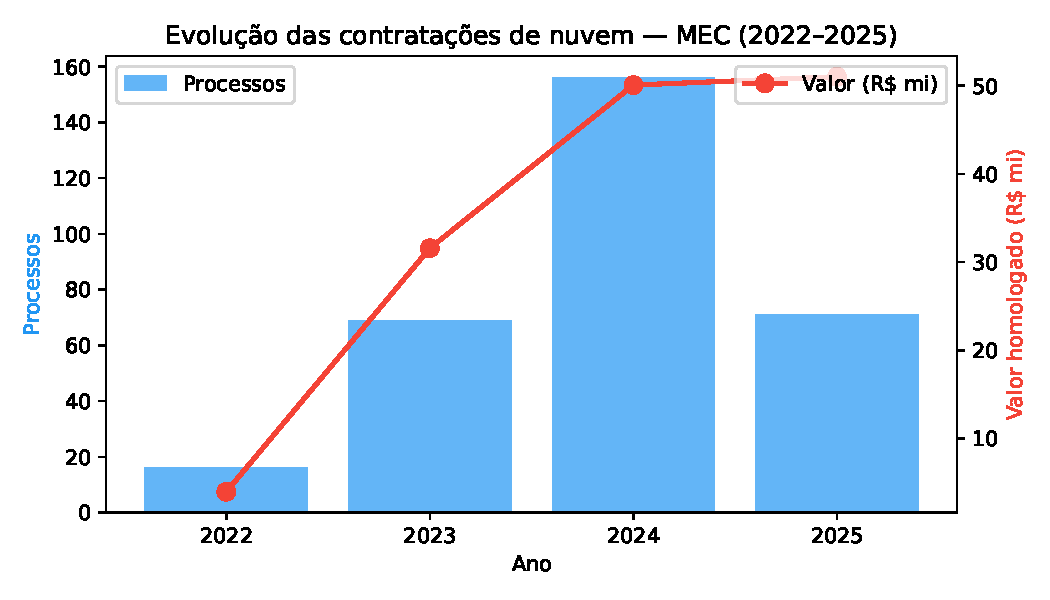
\includegraphics[width=0.85\textwidth]{assets/fig-evolucao.pdf}
\caption{Evolução temporal: processos (barras) e valor homologado (linha)}
\label{fig:evolucao}
\end{figure}

\begin{table}[ht]
\centering
\caption{Evolução temporal das contratações de nuvem}
\label{tab:evolucao}
\begin{tabular}{lrrr}
\toprule
\textbf{Ano} & \textbf{Processos} & \textbf{Valor homologado (R\$)} & \textbf{Instituições} \\
\midrule
2022 & 16 & \num{3958964} & 14 \\
2023 & 69 & \num{31578499} & 39 \\
2024 & 156 & \num{50070710} & 61 \\
2025 & 71 & \num{51013781} & 42 \\
2026 & 2 & \num{990619} & 2 \\
\bottomrule
\end{tabular}
\end{table}

\subsection{Custo de oportunidade da contratação direta (QP1)}

A Tabela~\ref{tab:economicidade} responde à QP1. O Pregão Eletrônico gera economicidade de 18,3\%, enquanto a Dispensa atinge apenas 5,3\% (diferença de 3,5$\times$). A Inexigibilidade apresenta economicidade nula (0,0\%), pois não há competição. A Concorrência Eletrônica alcança 11,3\%.

\begin{table}[ht]
\centering
\caption{Economicidade por modalidade de contratação}
\label{tab:economicidade}
\begin{tabular}{lrrrr}
\toprule
\textbf{Modalidade} & \textbf{n} & \textbf{Eco (\%)} & \textbf{Val. est. (R\$)} & \textbf{Val. hom. (R\$)} \\
\midrule
Pregão Eletrônico & 54 & 18,3 & \num{64767528} & \num{52909805} \\
Concorrência Eletrônica & 7 & 11,3 & \num{18312782} & \num{16241915} \\
Dispensa & 167 & 5,3 & \num{64573268} & \num{61149894} \\
Inexigibilidade & 42 & 0,0 & \num{3732015} & \num{3732015} \\
\bottomrule
\end{tabular}
\end{table}

O custo de oportunidade é expressivo: se os R\$ 64,6M em dispensas tivessem alcançado a mesma economicidade do Pregão (18,3\%), a economia adicional seria de aproximadamente R\$ 8,4M. Esse é um cenário hipotético superior, pois nem todos os objetos dispensados comportam certame competitivo (custos administrativos do Pregão podem superar a economia em processos de baixo valor). Ainda assim, o diferencial de 3,5$\times$ entre modalidades indica margem significativa para ganhos de eficiência.

A Figura~\ref{fig:boxplot} apresenta a dispersão dos valores homologados por modalidade, evidenciando que o Pregão concentra processos de maior valor com alta variabilidade, enquanto dispensas concentram-se na faixa inferior.

\begin{figure}[ht]
\centering
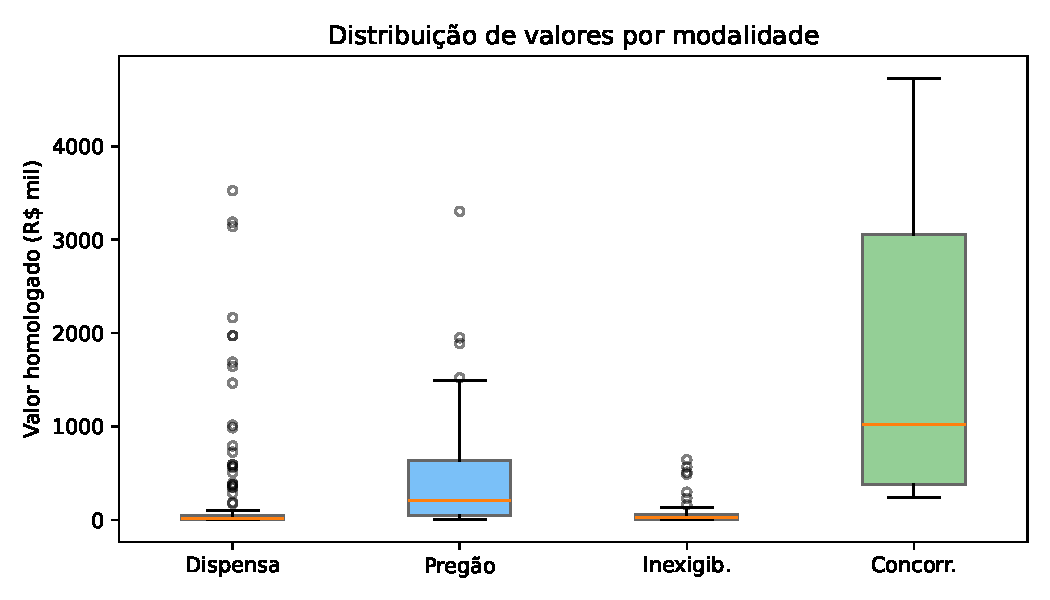
\includegraphics[width=0.85\textwidth]{assets/fig-boxplot.pdf}
\caption{Distribuição de valores homologados por modalidade (processos $\leq$ R\$ 5M)}
\label{fig:boxplot}
\end{figure}

\subsection{Recorrência de dispensas e oportunidades de consolidação (QP2)}

Foram identificadas 14 instituições com 3 ou mais dispensas de licitação para nuvem no mesmo exercício fiscal, totalizando R\$ 11,5 milhões em contratações diretas recorrentes. A Tabela~\ref{tab:fragmentacao} apresenta os casos mais expressivos.

\begin{table}[ht]
\centering
\caption{Instituições com maior recorrência de dispensas para nuvem (top 5)}
\label{tab:fragmentacao}
\begin{tabular}{lrrr}
\toprule
\textbf{Instituição} & \textbf{Ano} & \textbf{Dispensas} & \textbf{Valor (R\$)} \\
\midrule
CAU/BR & 2025 & 3 & \num{8767205} \\
UnB & 2024 & 6 & \num{1446977} \\
UFAM & 2025 & 3 & \num{773381} \\
IF (ES) & 2025 & 3 & \num{161376} \\
IF (outro) & 2025 & 4 & \num{105903} \\
\bottomrule
\end{tabular}
\end{table}

Destaque para a UnB com 6 dispensas no mesmo ano para objetos de nuvem, e o CAU/BR com 3 dispensas totalizando R\$ 8,7M. Esse valor já ultrapassaria o limite do Art. 75, II (R\$ 50.000), indicando provável uso do Art. 75, IX (empresa pública de TI). Esses padrões sugerem demandas recorrentes que poderiam se beneficiar de instrumentos como o Sistema de Registro de Preços.

Cabe observar que o CAU/BR (Conselho de Arquitetura e Urbanismo) consta no cadastro do Compras.gov.br como vinculado ao MEC (código 26000), mas trata-se de autarquia de fiscalização profissional sem relação com o ministério. Esse caso reforça os achados da QP3 sobre qualidade dos dados: inconsistências cadastrais na própria base de órgãos comprometem análises automatizadas e podem distorcer recortes institucionais.

\subsection{Qualidade dos dados do PNCP (QP3)}

A análise de integridade dos registros revela:

\begin{itemize}
\item \textbf{3,2\%} dos processos sem valor estimado cadastrado (zero ou nulo);
\item \textbf{12,1\%} sem valor de homologação (processo ainda em andamento ou omissão);
\item \textbf{1 outlier} com valor estimado superior a R\$ 1 bilhão (erro de cadastro com ordens de grandeza);
\item \textbf{0\%} de registros com valor homologado superior ao estimado (boa consistência nesse aspecto).
\end{itemize}

A ausência de 12,1\% dos valores de homologação compromete análises de economicidade e dificulta a auditoria automatizada. O outlier bilionário (presente nos totais brutos) distorce gravemente as médias se não tratado. Além disso, a base de órgãos do Compras.gov.br apresenta inconsistências de vinculação: ao menos uma autarquia (CAU/BR) consta como vinculada ao MEC sem relação institucional real, evidenciando que metadados cadastrais também carecem de validação.

\subsection{Especificidade técnica e economicidade (QP4)}

Para avaliar se a especificidade técnica dos Termos de Referência influencia a economicidade, aplicamos o teste de Mann-Whitney U (não paramétrico, adequado para distribuições assimétricas) sobre a economicidade individual de cada processo, agrupando em ``específicos'' (n=54, mencionam IaaS/PaaS/SaaS/provider) e ``genéricos'' (n=216).

\begin{itemize}
\item Específicos: mediana 0,0\%, média 9,1\%
\item Genéricos: mediana 0,0\%, média 11,6\%
\item Mann-Whitney $U = 5.964$, $p = 0{,}775$, $r_{rb} = -0{,}023$
\end{itemize}

O teste não rejeita $H_0$ ($p = 0{,}775 \gg 0{,}05$), com tamanho de efeito negligível ($r_{rb} = -0{,}023$). Conclui-se que \textbf{a especificidade técnica do objeto não influencia significativamente a economicidade obtida}. O fator determinante é a modalidade de contratação (competitiva vs. direta), não a precisão da descrição técnica. O tamanho amostral do grupo ``específicos'' (n=54) limita o poder estatístico do teste; estudos futuros com amostras maiores poderão confirmar esse resultado.

\subsection{Perfil institucional}

A distribuição por tipo de instituição revela: universidades federais lideram com 176 processos (56\%), seguidas por institutos federais (107 processos, 34\%) e outros (31, 10\%). A Figura~\ref{fig:uf} apresenta a distribuição geográfica.

Em termos de maturidade, as 10 instituições com mais processos de nuvem concentram 42\% do total (132/314), sugerindo forte heterogeneidade. Universidades de grande porte (UnB, UFMG, UFRJ) tendem a usar múltiplas modalidades, enquanto IFs menores recorrem quase exclusivamente a dispensas. Essa diferença indica que a capacidade operacional da equipe de TI (não apenas a demanda por nuvem) determina a escolha da modalidade.

\begin{figure}[ht]
\centering
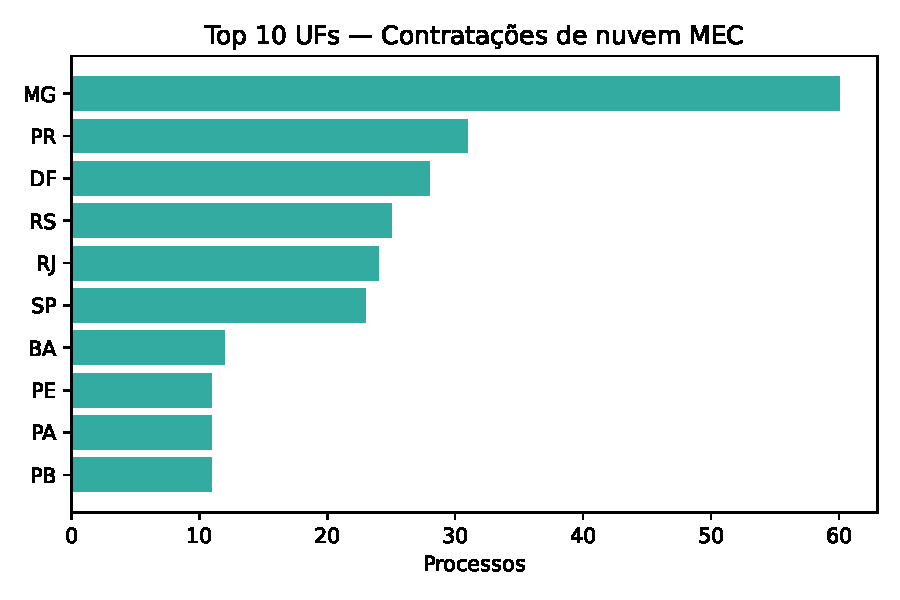
\includegraphics[width=0.75\textwidth]{assets/fig-uf.pdf}
\caption{Distribuição geográfica das contratações de nuvem (top 10 UFs)}
\label{fig:uf}
\end{figure}

O amparo legal nas 193 dispensas distribui-se em: Art. 75, II, contratações até R\$ 50.000 (129 processos, 66,8\%); Art. 75, IX, empresa pública de TI/SERPRO (37 processos, 19,2\%); Art. 75, XV, fundações de apoio (14 processos, 7,3\%); e outros incisos (13 processos, 6,7\%).

\section{Discussão}
\label{sec:discussao}

\subsection{O custo invisível da conveniência administrativa}

O diferencial de economicidade entre Pregão (18,3\%) e Dispensa (5,3\%) quantifica um ``custo de conveniência'' que a literatura anterior apenas apontava qualitativamente. Cada R\$ 1 milhão contratado via Dispensa em vez de Pregão representa aproximadamente R\$ 130.000 em economia não capturada. Esse resultado corrobora a Súmula TCU 269 sobre a necessidade de vincular contratações de TI a resultados mensuráveis \cite{tcu2020acordao1503}.

Cabe ressalvar que a métrica de economicidade depende da qualidade do valor estimado. Instituições que conduzem Pregão tendem a realizar pesquisas de preço mais rigorosas, o que pode resultar em estimativas mais realistas. Assim, parte do diferencial observado pode decorrer de estimativas infladas em dispensas, e não apenas de competição real. Ainda assim, o resultado de Baldi e Vannoni \cite{baldi2018econometric} em contexto distinto (Forças Armadas espanholas) encontrou magnitude comparável, reforçando a robustez do achado.

A inexigibilidade (economicidade 0\%) é esperada e não constitui anomalia. Processos com SERPRO/Dataprev são precificados via tabela institucional. Contudo, os 37 processos via Art. 75, IX merecem atenção: embora legalmente amparados, representam concentração de mercado em um fornecedor estatal sem incentivo competitivo.

\subsection{Recorrência de dispensas: oportunidade de consolidação}

A existência de 14 instituições com 3 ou mais dispensas para nuvem no mesmo ano pode refletir: (i) objetos genuinamente distintos; (ii) demandas que surgem ao longo do exercício sem planejamento consolidado; ou (iii) limitações operacionais para conduzir certames em tempo hábil. O manual do TCU \cite{tcu2024licitacoes} destaca a importância da ``análise quanto à vantajosidade técnica e econômica do parcelamento'', recomendando a consolidação quando houver objetos similares. O Instrumento de Padronização AGU/MGI \cite{agu2023padronizacao} reforça que o modelo de contratação de nuvem deve priorizar SRP quando houver ``necessidade de contratações permanentes ou frequentes''. Esse é o perfil típico de serviços de nuvem.

O caso da UnB (6 dispensas, R\$ 1,4M) ilustra o padrão. Cada dispensa pode estar dentro dos limites legais, mas a consolidação em um Pregão poderia gerar economia de 18,3\% (R\$ 265.000) e reduzir o esforço administrativo. O CAU/BR (R\$ 8,7M em 3 dispensas) provavelmente utiliza o Art. 75, IX (empresa pública de TI). Está amparado legalmente, mas sem o benefício da competição.

O Decreto nº 11.462/2023 \cite{brasil2022decreto11462}, que regulamenta o SRP sob a Lei 14.133/2021, prevê expressamente sua adoção ``quando for conveniente a aquisição de bens com previsão de entregas parceladas ou contratação de serviços remunerados por unidade de medida''. Essa descrição se enquadra perfeitamente em créditos de nuvem e subscrições. O uso marginal de 9,9\% de SRP no dataset confirma oportunidade perdida de consolidação.

Iniciativas de consolidação já estão em curso. A SGD/MGI conduziu sucessivas versões de contratação centralizada para o SISP, culminando no ``Nuvem 3.0'': estratégia multinuvem com múltiplos catálogos e integradores habilitados a ofertar no mínimo três provedores \cite{sgd2024etp_nuvem3, brasil2023portaria5950}. A Nuvem de Governo, operada pelo Serpro, consolidou-se como infraestrutura soberana para dados sensíveis. No âmbito das autarquias, instituições como o IFSP conduzem credenciamentos próprios de integradores (Art. 79, III, Lei 14.133/2021, mercado fluido) \cite{ifsp2026credenciamento}. O modelo reconhece que instituições de ensino têm demandas recorrentes e heterogêneas de TIC: ensino, pesquisa, extensão e rotinas administrativas geram necessidade contínua de novos serviços de nuvem. A competição ocorre na fase de execução, a cada Ordem de Serviço. Esses movimentos convergem para o mesmo objetivo: consolidar demandas pulverizadas em instrumentos que equilibrem agilidade e economicidade.

\subsection{PNCP como instrumento de auditoria: potencial e limitações}

A taxa de 12,1\% de registros sem homologação limita a capacidade de auditoria automatizada. Mais criticamente, a API do PNCP não disponibiliza dados de fornecedor no endpoint de publicação, impossibilitando análises de concentração de mercado (HHI) que seriam fundamentais para avaliar riscos de \textit{lock-in} tecnológico.

A presença de outlier bilionário confirma a necessidade de validação na entrada de dados. Essa é uma recomendação prática para a equipe do PNCP.

\subsection{Maturidade heterogênea e o ``abismo digital''}

O fato de 55\% das autarquias do MEC não registrarem nenhuma contratação de nuvem no PNCP evidencia heterogeneidade significativa. Três explicações são possíveis: (i) essas instituições mantêm infraestrutura \textit{on-premises}; (ii) contratam via adesão a atas de outros órgãos (não registrada individualmente); ou (iii) ainda não adotaram soluções de nuvem.

\subsection{Ameaças à validade}

\textbf{Interna:} a classificação por palavras-chave pode gerar falsos negativos (descrições genéricas como ``serviços de TI'') e falsos positivos (menção incidental). \textbf{Externa:} resultados específicos ao recorte MEC; outros ministérios podem apresentar padrões distintos. \textbf{Construto:} o PNCP foi instituído em 2021, e a adesão nos primeiros anos foi parcial.

\subsection{Aderência à Portaria SGD/MGI nº 5.950/2023}

A Portaria 5.950/2023 \cite{brasil2023portaria5950} exige classificação por camada (IaaS/PaaS/SaaS), modelos de remuneração padronizados e priorização de SRP. No dataset, apenas 20,7\% dos processos (65/314) mencionam explicitamente camada ou provedor. Os demais 79,3\% usam descrições genéricas (``nuvem'', ``hospedagem'', ``cloud''). O uso de SRP é de apenas 9,9\%. Dos 156 processos de 2024 (posteriores à Portaria, de outubro/2023), a predominância de descrições genéricas persiste.

Esses dados sugerem baixa aderência, mas com ressalva: os campos do PNCP são texto livre e não permitem verificar a existência de planilhas de custo ou modelos de remuneração nos TRs completos. A inferência é, portanto, uma proxy. Estudos futuros com acesso aos TRs integrais poderão confirmar a extensão da não-conformidade.

\section{Conclusão}
\label{sec:conclusao}

Este estudo apresentou o primeiro diagnóstico quantitativo das contratações de nuvem nas autarquias do MEC com dados do PNCP, respondendo às quatro questões de pesquisa propostas:

\begin{itemize}
\item \textbf{QP1:} O custo de oportunidade da contratação direta é de 13 pontos percentuais de economicidade perdida (5,3\% vs. 18,3\%), estimado em R\$ 8,4M para o dataset analisado.
\item \textbf{QP2:} 14 instituições apresentam recorrência de dispensas (R\$ 11,5M no mesmo exercício), sinalizando oportunidades concretas de consolidação via SRP ou certame competitivo.
\item \textbf{QP3:} O PNCP apresenta 12,1\% de registros incompletos e não disponibiliza dados de fornecedor via API, limitando auditoria automatizada.
\item \textbf{QP4:} A especificidade técnica do TR não influencia significativamente a economicidade (Mann-Whitney $p = 0{,}775$). O fator determinante é a modalidade competitiva.
\end{itemize}

Adicionalmente, a confrontação com a Portaria SGD/MGI nº 5.950/2023 revelou que 79,3\% dos processos não classificam o serviço nas camadas IaaS/PaaS/SaaS exigidas pela norma, e apenas 9,9\% utilizam SRP, indicando baixa aderência ao modelo institucionalizado.

\subsection{Implicações práticas}

Para gestores de TI, a consolidação via SRP pode gerar economia de até 18,3\%. Recomenda-se avaliar adesão a atas existentes antes de iniciar contratações individuais. Para a SGD/MGI, a baixa aderência à Portaria 5.950/2023 (79,3\% sem classificação por camada) sugere necessidade de capacitação e modelos padronizados de TR.

Para o PNCP, a inclusão de campos estruturados (tipo de serviço, fornecedor, modelo de remuneração) e validação de valores na entrada melhorariam a auditabilidade. Para órgãos de controle, o indicador de recorrência (3+ dispensas/ano/instituição) pode ser automatizado em dashboards de acompanhamento.

\subsection{Trabalhos futuros}

\begin{enumerate}
\item Extensão do recorte para todos os ministérios e coleta de dados de fornecedores (HHI), viabilizando análise de concentração de mercado.
\item Análise textual dos TRs completos com NLP para classificação por camada e verificação de conformidade com a Portaria 5.950/2023.
\item Estudo longitudinal após maturação do PNCP (previsão: 2027), com cobertura temporal homogênea.
\end{enumerate}

\bibliographystyle{plain}
\bibliography{references}

\end{document}
